% This is samplepaper.tex, a sample chapter demonstrating the
% LLNCS macro package for Springer Computer Science proceedings;
% Version 2.20 of 2017/10/04
%
\documentclass[runningheads]{llncs}
%
\usepackage{graphicx}
\usepackage{amsmath}
\usepackage{amsfonts}
\usepackage{float}
% Used for displaying a sample figure. If possible, figure files should
% be included in EPS format.
%
% If you use the hyperref package, please uncomment the following line
% to display URLs in blue roman font according to Springer's eBook style:
% \renewcommand\UrlFont{\color{blue}\rmfamily}

\hyphenation{re-pre-sent}
\hyphenation{mo-dels}
\hyphenation{do-cu-ments}
\hyphenation{di-gi-tal}
\hyphenation{per-cep-tually}
\hyphenation{wa-ter-mar-king}
\hyphenation{ca-mou-fla-ged}
\hyphenation{Approach}
\hyphenation{qua-li-ty}
\hyphenation{mo-di-fying}
\hyphenation{pro-per-ty}
\hyphenation{mi-ni-mum}
\hyphenation{pa-ra-me-ters}
\hyphenation{using}
\begin{document}
%
\title{{Watermarking based on Krawtchouk moments for handwritten document images}}
%
%\titlerunning{Abbreviated paper title}
% If the paper title is too long for the running head, you can set
% an abbreviated paper title here
%
\author{Ernesto Avila-Domenech \and Anier Soria-Lorente}
%
\authorrunning{E. Avila-Domenech et al.}
% First names are abbreviated in the running head.
% If there are more than two authors, 'et al.' is used.
%
\institute{Universidad de Granma, Carretera Central v{\'i}a Holgu{\'i}n Km $\frac{1}{2}$, Granma, Cuba \email{\{eadomenech, asorial1983\}@gmail.com}\\	}
%
\maketitle              % typeset the header of the contribution
%
\begin{abstract}
In this paper, a digital watermarking technique for copyright protection based on the concept of embed a digital watermark and modifying coefficients in Krawtchouk moments domain is presented. This technique is specifically for handwritten document images using a QR code as a digital watermark. It consists in dividing the image into $8\times 8$ pixels blocks, where the number of selected blocks is equal to the number of watermark bits. The Krawtchouk moments of each selected block are determined. After that, one coefficient is modified using Dither modulation. In addition, the results obtained in terms of perceptual quality (PSNR) and robustness (BER) show that the proposed technique is robust to JPEG compression attacks keeping imperceptibility.

\keywords{Digital watermarking \and Genetic algorithm \and Hadwritten documents \and Krawtchouk moments \and QR code.}
\end{abstract}
%
%
%
\section{Introduction}
The rapid evolution of the digital world has facilitated the manipulation and
transmission of digital media, such as text, images, audio, video and 3D models. Easy access and replication have led to serious problems with copyright protection of media. Therefore, the scientific community has developed several techniques to ensure the protection of copyright and the information in general.

	One of the more used techniques in the Information Hiding field is the Digital watermarking. It is defined as the process of embedding	information  into  a  noise-tolerant  digital  signal to  identify  the  copyright  ownership  of the  media \cite{nin2013digital}.
	
	There  is  an  extensive literature about watermarking techniques applied to various types of host content, such as audio \cite{Ali2017,Dhar2017}, image \cite{Ghazvini2017,Juarez-sandoval2018,Su2017} and video \cite{sake2018bi}.
	
	Recently, the scientists developed the orthogonal moments, which use as kernel functions orthogonal polynomials that constitute orthogonal basis. This property of orthogonality, gives to the corresponding moments the feature of minimum information redundancy, meaning that different moment orders describe different image content. Some representative moment families are the Tchebichef, dual Hahn, Racah and Krawtchouk moments \cite{papakostas2010computation}.
	
	The main advantage of the orthogonal moments is their ability to uniquely describe the content of an image by permitting the full reconstruction of the image they describe. The information embedment through moments' domain in conjunction with the minimum reconstruction error of the final watermarked image, makes image moments an attractive and useful tool in watermarking applications \cite{Papakostas2014}.
	
	In this paper, we propose a new digital watermarking schema based on the set of Krawtchouk moments. The rest of the paper is organized as follows. Section 2 covers the background of this work in three subsections. The approaches followed in the proposed system are discussed in Section 3. Finally, experimental results and discussions are given in Section 4.
\section{Background}

\subsection*{Arnold transform}
The Arnold transform is a invertible method that can be used for pixel scrambling, and has been adopted in various watermarking schemes. By using the Arnold transform, the high pixel correlation can be disrupted. The Arnold transform is shown in Eq.~\ref{Arnold}, where $p$ and $q$ are positive integers, $det(A) = 1$, and $(x', y')$ are the new coordinates of the pixel after Arnold transform is applied to a pixel at position $(x, y)$ \cite{Chow2017}. The
transform changes the position of two pixels, and if it is done several times, a disordered image can be generated. Because of Arnold transform of periodicity, the original image will be recovered.
\begin{equation}
\left[\begin{array}{c}x'\\y'\end{array}\right]=A\left[\begin{array}{c}x\\y\end{array}\right]\ mod\ N=\left[\begin{array}{cc}1 & p\\q & pq+1\end{array}\right]\left[\begin{array}{c}x\\y\end{array}\right]\ mod\ N.
\label{Arnold}
\end{equation}
In Fig.~\ref{AT}, on the left, original watermark, in the center, scrambled watermark image using Arnold transform $20$ times (with $p=1$, $q=1$ and $N=62$) and  in the right, the recovered watermark image using Arnold transform $10$ times more because for $N=62$ the periodicity is $30$.
\begin{figure}
	\begin{center}
		\begin{tabular}{|c|c|c|}\hline
			\includegraphics[width=0.15\textwidth]{Watermarking.png}
			&\includegraphics[width=0.15\textwidth]{Watermarking20.png}
			&\includegraphics[width=0.15\textwidth]{Watermarking30.png}\\\hline
		\end{tabular}
	\end{center}
	\caption{Watermark image, scrambled image and recovered image.}
	\label{AT}
\end{figure}
\subsection*{Krawtchouk moments}
The Krawtchouk moments were introduced by Yap in \cite{Yap2003}. These orthogonal moments satisfy the following recurrence relation
\begin{multline*}
\alpha_n(Np-2np+n-x)\overline{K}_{n}^{p,N}(x) \\= p(n-N)\overline{K}_{n+1}^{p,N}(x)+\beta_n n(1-p)\overline{K}_{n-1}^{p,N}(x),\quad n\geq 1,
\end{multline*}
with initial conditions 
\begin{equation*}
\overline{K}_{0}^{p,N}(x) = \sqrt{w^{p,N}(x)p^{-1}},
\end{equation*}	
and
\begin{equation*}
\overline{K}_{1}^{p,N}(x) = (Np-x)(Np)^{-1}\sqrt{w^{p,N}(x)(1-p)(Np)^{-1}},
\end{equation*}
where $\alpha_n = \sqrt{\frac{(1-p)(n+1)}{p(N-n)}}$, $\beta_n = \sqrt{\frac{(1-p)^2(n+1)n}{p^2(N-n)_2}}$, $w^{p,N}(x) = \binom{N}{x}p^x(1-p)^{N-x}$ and $0<p<1$.

The Krawtchouk moment of order $(m+n)$ of an image $f(x,y)$ with $M\times N$ pixels is defined as

\begin{equation}
K_{mn}=\sum_{x=0}^{M-1}\sum_{y=0}^{N-1}f(x,y)\overline{K}_{m}^{p,M}(x)\overline{K}_{n}^{q,N}(y),
\label{DKT}
\end{equation}
where $m\in \left[ 0,M-1\right] $ and $n\in \left[ 0,N-1\right] $.

The image $f(x,y)$ can be reconstructed using
\begin{equation}
f(x,y)=\sum_{m=0}^{M-1}\sum_{n=0}^{N-1}K_{mn}\overline{K}_{m}^{p,M}(x)\overline{K}_{n}^{q,N}(y),
\label{IDKT}
\end{equation}
where $x\in \left[ 0,M-1\right] $ and $y\in \left[ 0,N-1\right] $.

The lower order Krawtchouk moments store information of a specific region-of-interest of an image, the higher order moments store information of the rest of the image. Therefore, by reconstructing the image from the lower order moments and discarding the higher order moments, a sub-image can be extracted from the subject image. For each additional moment used in reconstructing the image, the square error of the reconstructed image is reduced \cite{Yap2003}.

	The set of lower order Krawtchouk moments is generally the set of perceptually significant components of the image. This choice ensures that the watermark is robust to attacks \cite{Yap2004}.
\subsection*{Dither modulation quantization}
Dither modulation quantization technique is one of the most popular in the watermarking. It has good performance on following requirements of watermarking: perceptibility ratio, data payload, robustness, and blind extraction. The combination of dither modulation quantization with different transformation domain watermarking methods also improves watermark extraction capability \cite{chen2001quantization}. 

	One bit of the watermark can be embedded as
\begin{equation}
|C{}_{0}^{'}(k_{1},k_{2})|=\begin{cases}
2\Delta\times round(\frac{|C{}_{0}(k_{1},k_{2})|}{2\Delta})+\frac{\Delta}{2}, & if\:W(i,j)=1\\
2\Delta\times round(\frac{|C{}_{0}(k_{1},k_{2})|}{2\Delta})-\frac{\Delta}{2} & if\:W(i,j)=0
\end{cases},
\label{DMEm}
\end{equation}
where $\Delta$ is the quantization step controlling the embedding strength of the watermark bit, $|\cdot|$ is the absolute operator, $round(\cdot)$ denotes the rounding operation to the nearest integer, $W(i,j)$ is the watermark bit at the position $(i,j)$ and $C{}_{0}^{'}(k_{1},k_{2})$ is the modified block.

	To extract the watermark it is used
\begin{equation}
W^{*}(i,j)=arg_{\sigma\in\{0,1\}}min(|C_{0}^{''}(k_{1},k_{2})|_{\sigma}-|C_{0}^{*}(k_{1},k_{2})|)
\label{DMEx},
\end{equation}
where $C_{0}^{*}(k_{1},k_{2})$ is the extracted watermark and $|C_{0}^{''}(k_{1},k_{2})|_{\sigma}$ is defined as
\begin{equation}
|C_{0}^{''}(k_{1},k_{2})|_{\sigma}=\begin{cases}
2\Delta\times round(\frac{|C_{0}^{*}(k_{1},k_{2})|}{2\Delta})+\frac{\Delta}{2}, & if\:\sigma=1\\
2\Delta\times round(\frac{|C_{0}^{*}(k_{1},k_{2})|}{2\Delta})-\frac{\Delta}{2} & if\:\sigma=0
\end{cases}.
\end{equation}
\section{Materials and methods}\label{metodos}
\subsection*{Watermark embedding scheme}
\begin{itemize}
	\item[\checkmark] The binary watermark image (QR code) is scrambled using Arnold transform (see Eq.~\ref{AT}).
	\item[\checkmark] The cover image is transformed from RGB to YCbCr color space, and the Y component, corresponding to the luminance information, is divided into small image blocks of $8\times 8$ pixels.
	\item[\checkmark] The Krawtchouk moments of selected blocks are determined by Eq.~\ref{DKT}.
	\item[\checkmark] Watermark bit is embedded in the selected block moments using Dither modulation (see Eq.~\ref{DMEm}).
	\item[\checkmark] Watermarked blocks can be obtained using Eq.~\ref{IDKT}.
	\item[\checkmark] The last step is to transform the YCbCr to RGB space to obtain RGB watermarked image.
\end{itemize}
\begin{figure}[H]
	\begin{center}
			\includegraphics[width=1.1\textwidth]{WP.png}
	\end{center}
	\caption{Watermark embedding and extraction scheme.}
	\label{PIE}
\end{figure}
\subsection*{Watermark extraction}
\begin{itemize}
	\item[\checkmark] The watermarked image is transformed from the RGB to the YCbCr color space and the Y component is divided into $8\times 8$ pixels blocks.
	\item[\checkmark] The Krawtchouk moments of selected blocks are determined.
	\item[\checkmark] Scrambled watermark bits are obtained with the selected block moments using Dither modulation (see Eq.~\ref{DMEx}).
	\item[\checkmark] Finally, QR code watermark is constructed with the scrambled bits using Arnold transform.
\end{itemize}
\subsection*{Optimization against JPEG compression attacks}
Recently, metaheuristic optimization algorithms have been used \cite{Abdelhakim2018,Avila-Domenech1899} to improve the performance of watermarking methods in solving the conflict between quality and robustness. Metaheuristic algorithms are used to find parameters that can be used to increase robustness but maintaining the imperceptibility parameters. Some watermarking methods use the metaheuristic algorithm to optimize a single objective, such as robustness or quality, while the other objective is considered through predetermined inclusion parameters or evaluated in an adaptive way.
\begin{figure}[h]
	\begin{center}
		\begin{tabular}{|c|c|}\hline
			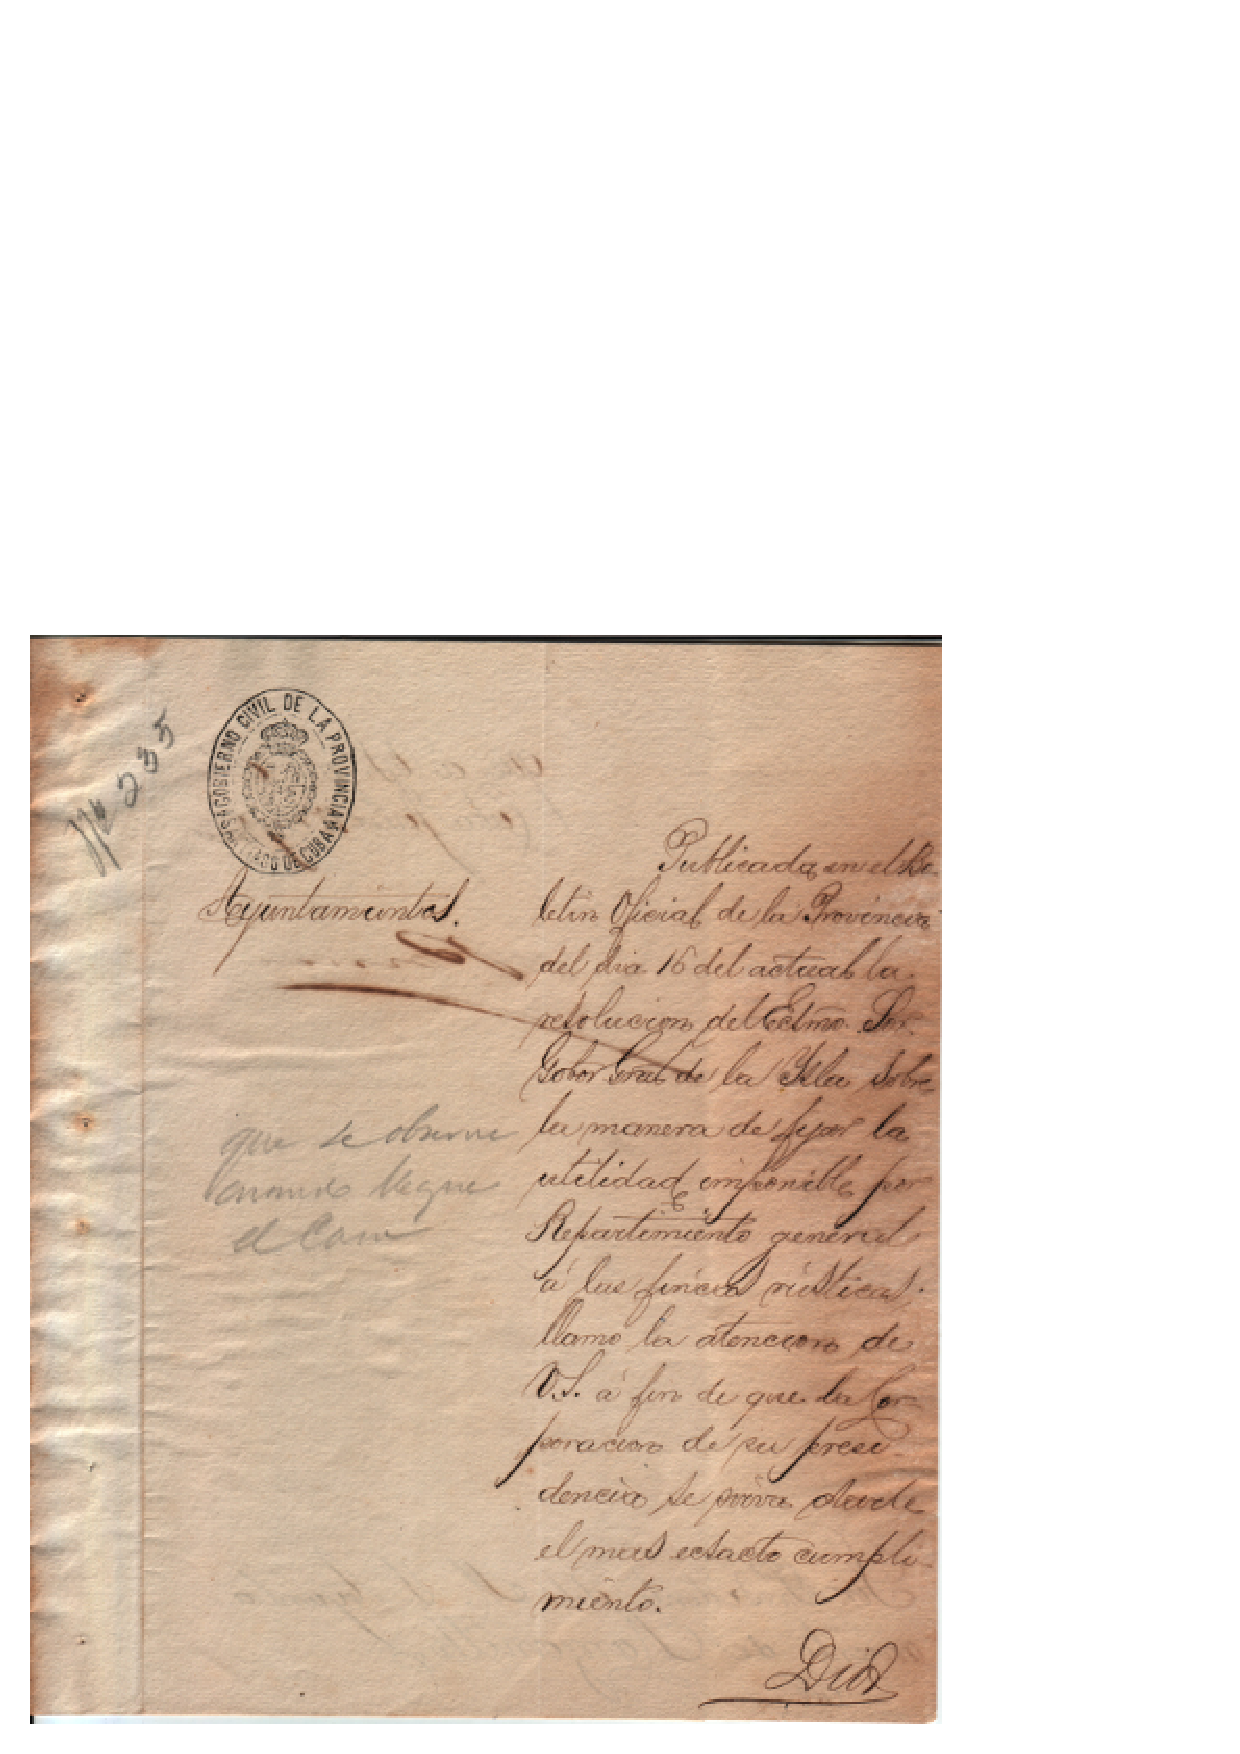
\includegraphics[width=0.20\textwidth]{1.jpg}
			&\includegraphics[width=0.20\textwidth]{8.jpg}\\\hline
		\end{tabular}
	\end{center}
	\caption{Handwritten document images (1.jpg and 2.jpg, left to right).}
	\label{img_of_AHM}
\end{figure}

In this proposal, using the images represented in Fig.~\ref{img_of_AHM}, a similar genetic algorithm as the one used in \cite{Avila-Domenech1899} was applied to determine the ideal parameters with the purpose of guaranteeing the performance between imperceptibility and robustness.

\begin{table}
	\centering
	\begin{tabular}{|c|c|c|c|c|c|c|}
		\hline
		Attack & FA & Coefficient & $\Delta$ & PSNR & BER & QR decoded \\\hline
		JPEG 75\% & 0.829307 & 43 & 35 & 54.0657677342 & 0.00104058272633 & Yes \\
		JPEG 50\% & 0.817445 & 43 & 72 & 49.2058749843 & 0.00520291363163 & Yes \\
		JPEG 20\% & 0.805757 & 19 & 128 & 43.2630691126 & 0.00312174817898 & Yes \\
		Guetzli 85\% \cite{Alakuijala2017} & 0.819719 & 28 & 49 & 49.4777158275 & 0.0 & Yes \\
		\hline
	\end{tabular}
	\caption{Optimized parameters for 1.jpg image.}
\end{table}
\begin{table}
	\centering
	\begin{tabular}{|c|c|c|c|c|c|c|c|}
		\hline
		Attack & FA & Coefficient & $\Delta$ & PSNR & BER & QR decoded \\\hline
		JPEG 75\% & 0.826590 & 43 & 35 & 53.9286245147 & 0.00728407908429 & Yes \\
		JPEG 50\% & 0.809593 & 43 & 75 & 48.4338108172 & 0.0239334027055 & Yes \\
		JPEG 20\% & 0.804583 & 19 & 141 & 42.5328352352 & 0.00208116545265 & Yes \\
		Guetzli 85\% \cite{Alakuijala2017} & 0.819719 & 28 & 49 & 49.4777158275 & 0.0 & Yes \\
		\hline
	\end{tabular}
	\caption{Optimized parameters for 2.jpg image.}
\end{table}
In the parameters obtained for both images, the coefficient to be used is the same as the applied attack. It can be observed that in the JPEG $20\%$ attack, the optimum coefficient to be used for both images is $19$ and $\Delta$ for one case is $128$ and in other case $141$. Taking into account the four attacks, the one with the $20\%$ is the most aggressive, the $19$ coefficient is taken as reference because it is the same for both images. Considering that the bit error rate generates acceptable values, $128$ is considered as $\Delta$ value, because it is the lowest value for JPEG $20\%$ attack in both images.                      

\section{Results and Discussion}
For the evaluation of results the logarithmic value of ratio between signal and noise (PSNR), and the bit error rate (BER) are used.

	The PSNR value is calculated using the equation
\begin{equation}
PSNR=10\log_{10}\left(\frac{MAX^{2}}{MSE}\right)=20\log_{10}\left(\frac{MAX}{\sqrt{MSE}}\right),
\label{equation_psnr}
\end{equation}
where $MAX$ is the maximum possible pixel value of the image and $MSE$
represent a mean square error.
\begin{equation}
MSE=\frac{1}{MN}\sum_{i=1}^{M}\sum_{j=1}^{N}\left[f'(m,n)-f(m,n)\right]^{2},
\end{equation}
where $M\times N$ is the size of the image, $f(m,n)$ is a cover image and $f'(m,n)$ is a watermarked image.

The BER value is calculated using the equation
\begin{equation}
BER=\frac{1}{B}\sum_{n=0}^{B-1}
\begin{cases}
1 & \mbox{if }\, w'(n)\neq w(n)\\
0 & \mbox{if }\, w'(n)=w(n)
\end{cases}
\label{ber},
\end{equation}
where $w(n)$ y $w'(n)$ are binary bits (0 or 1) of the original watermark and extracted watermark. $B$ is the number of pixels of the watermark.
	
	With the optimized parameters, $60$ images that belong to \cite{fischer2011transcription} were evaluated. The values obtained  for all images were acceptable because in $100\%$ of cases the watermark was decoded. Besides the PSNR values were between $44dB$ and $46dB$ (see Fig.~\ref{psnr}), it means the nonexistence of visual differences between the watermarked and original images. Moreover, Fig.~\ref{ber} shows the obtained result for BER corresponding to these images for the four types of JPEG compression attacks. As it can be observed, values under $0.005 \%$ were achieved, being decoded all QR watermark codes.	
\begin{figure}[t]	% h-here, t-top, b-bottom
	\begin{center}
		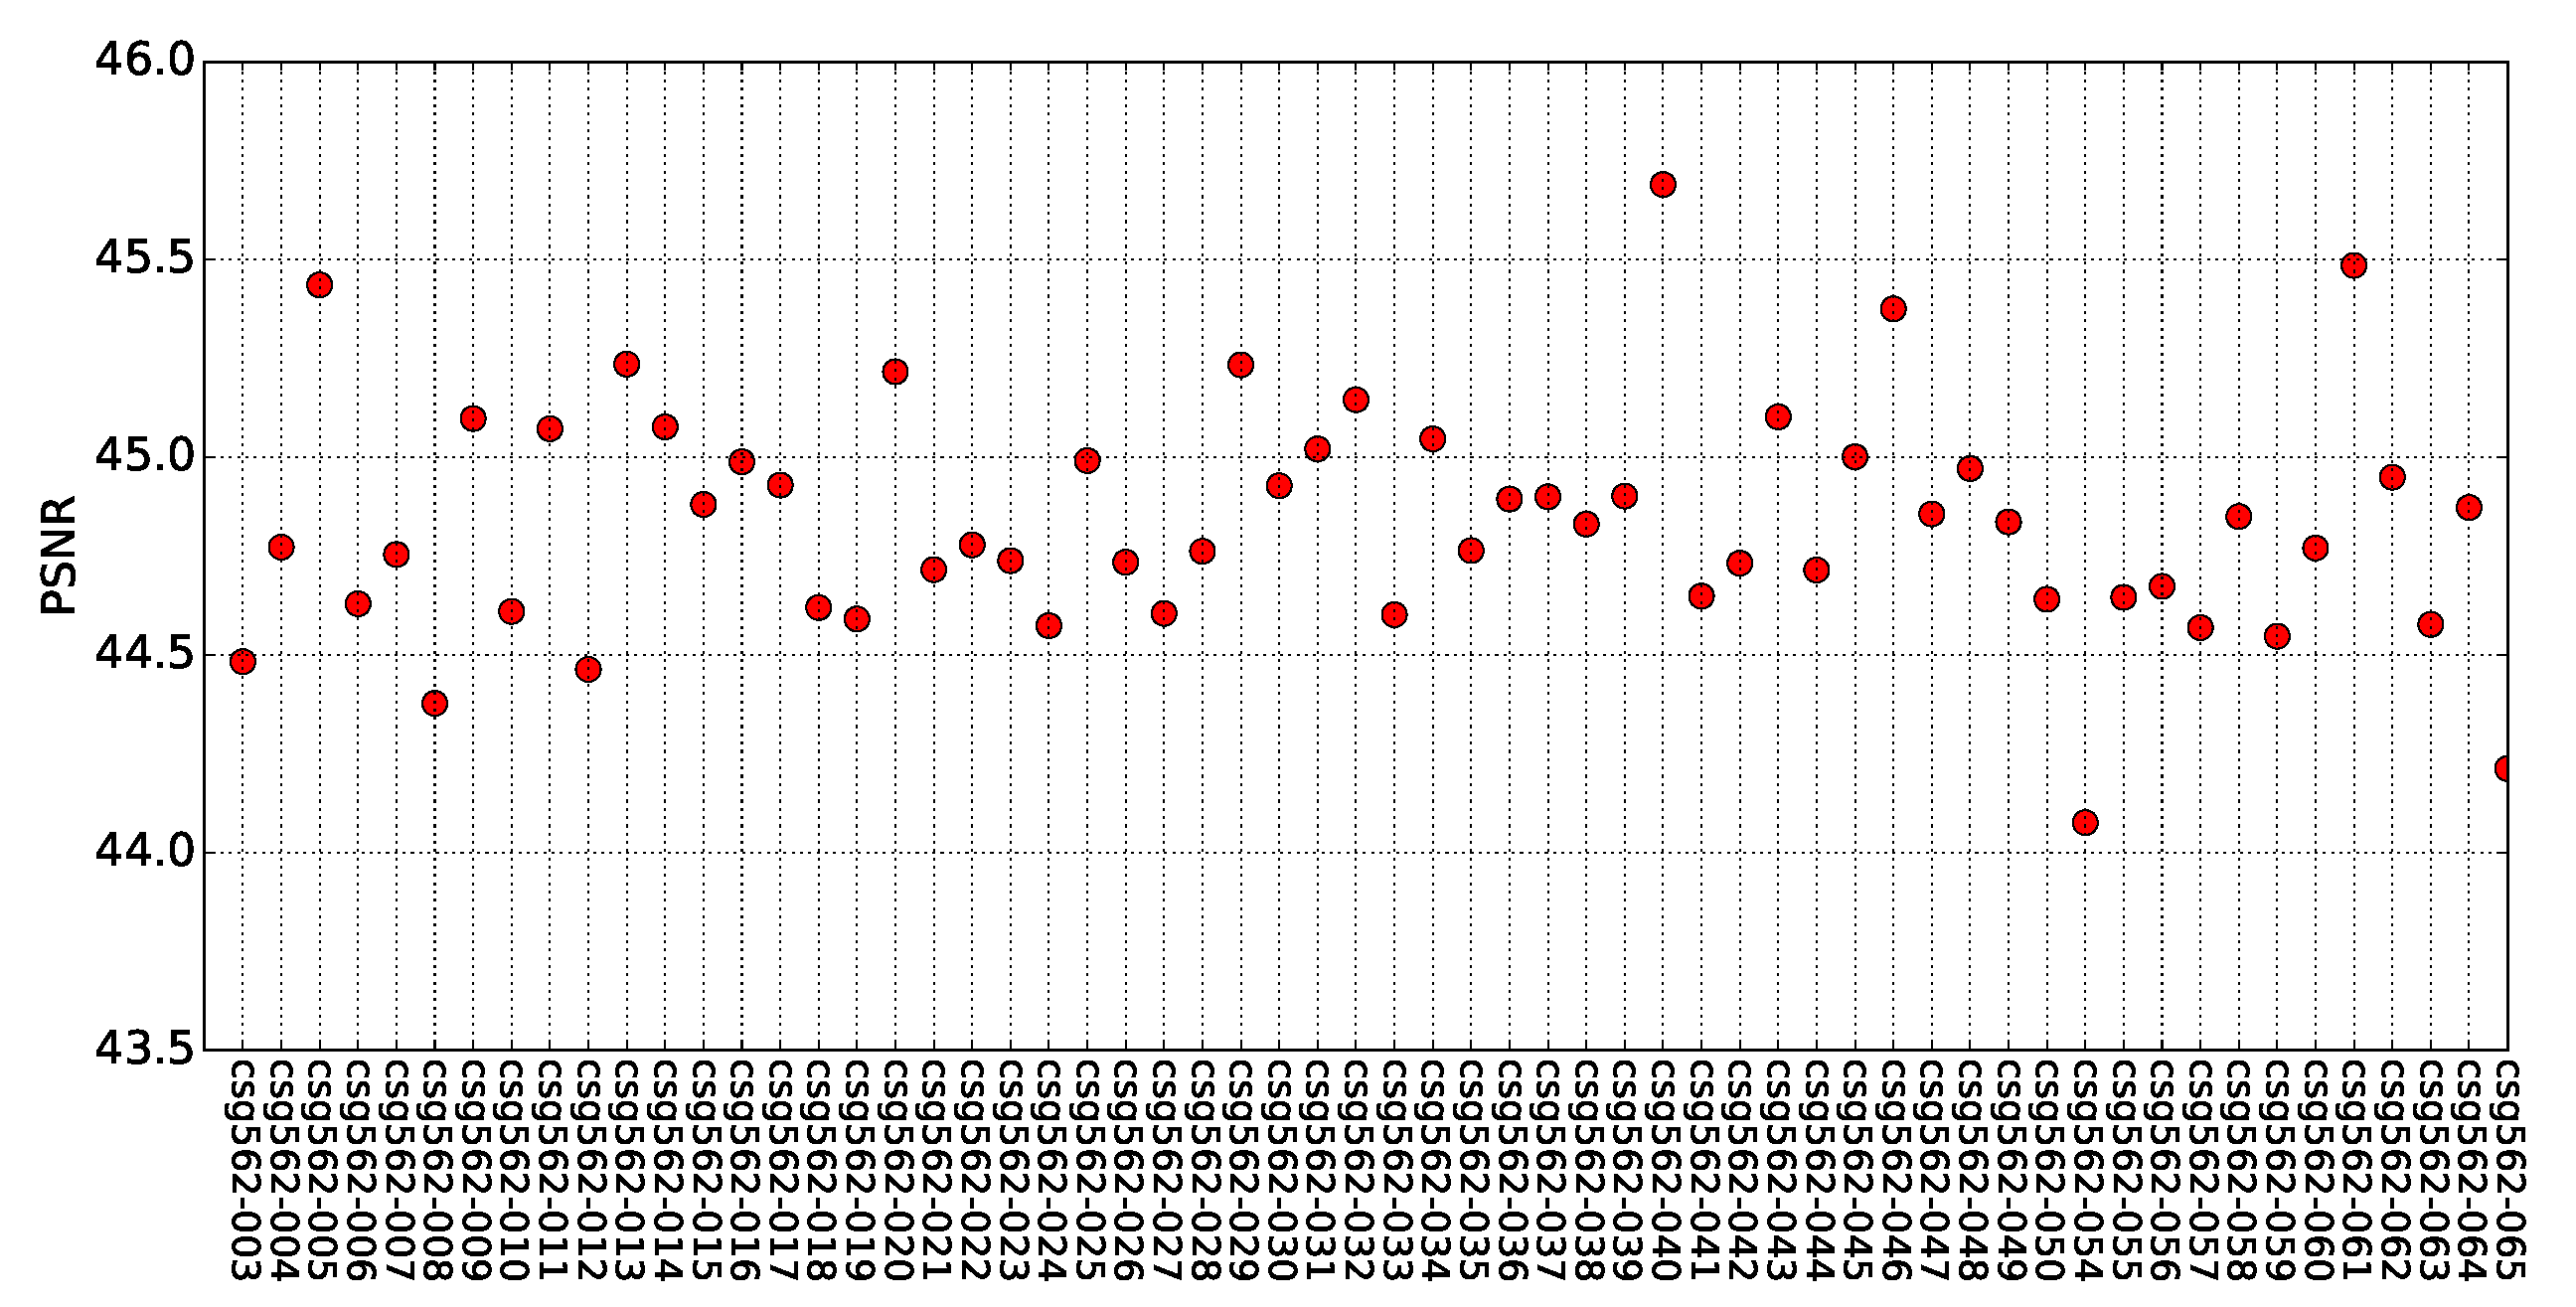
\includegraphics[width=0.86\textwidth]{psnr.eps}
	\end{center}
	\caption{PSNR values for Saint Gall database watermarked images.}
	\label{psnr}
\end{figure}
\begin{figure}[H]	% h-here, t-top, b-bottom
	\begin{center}
			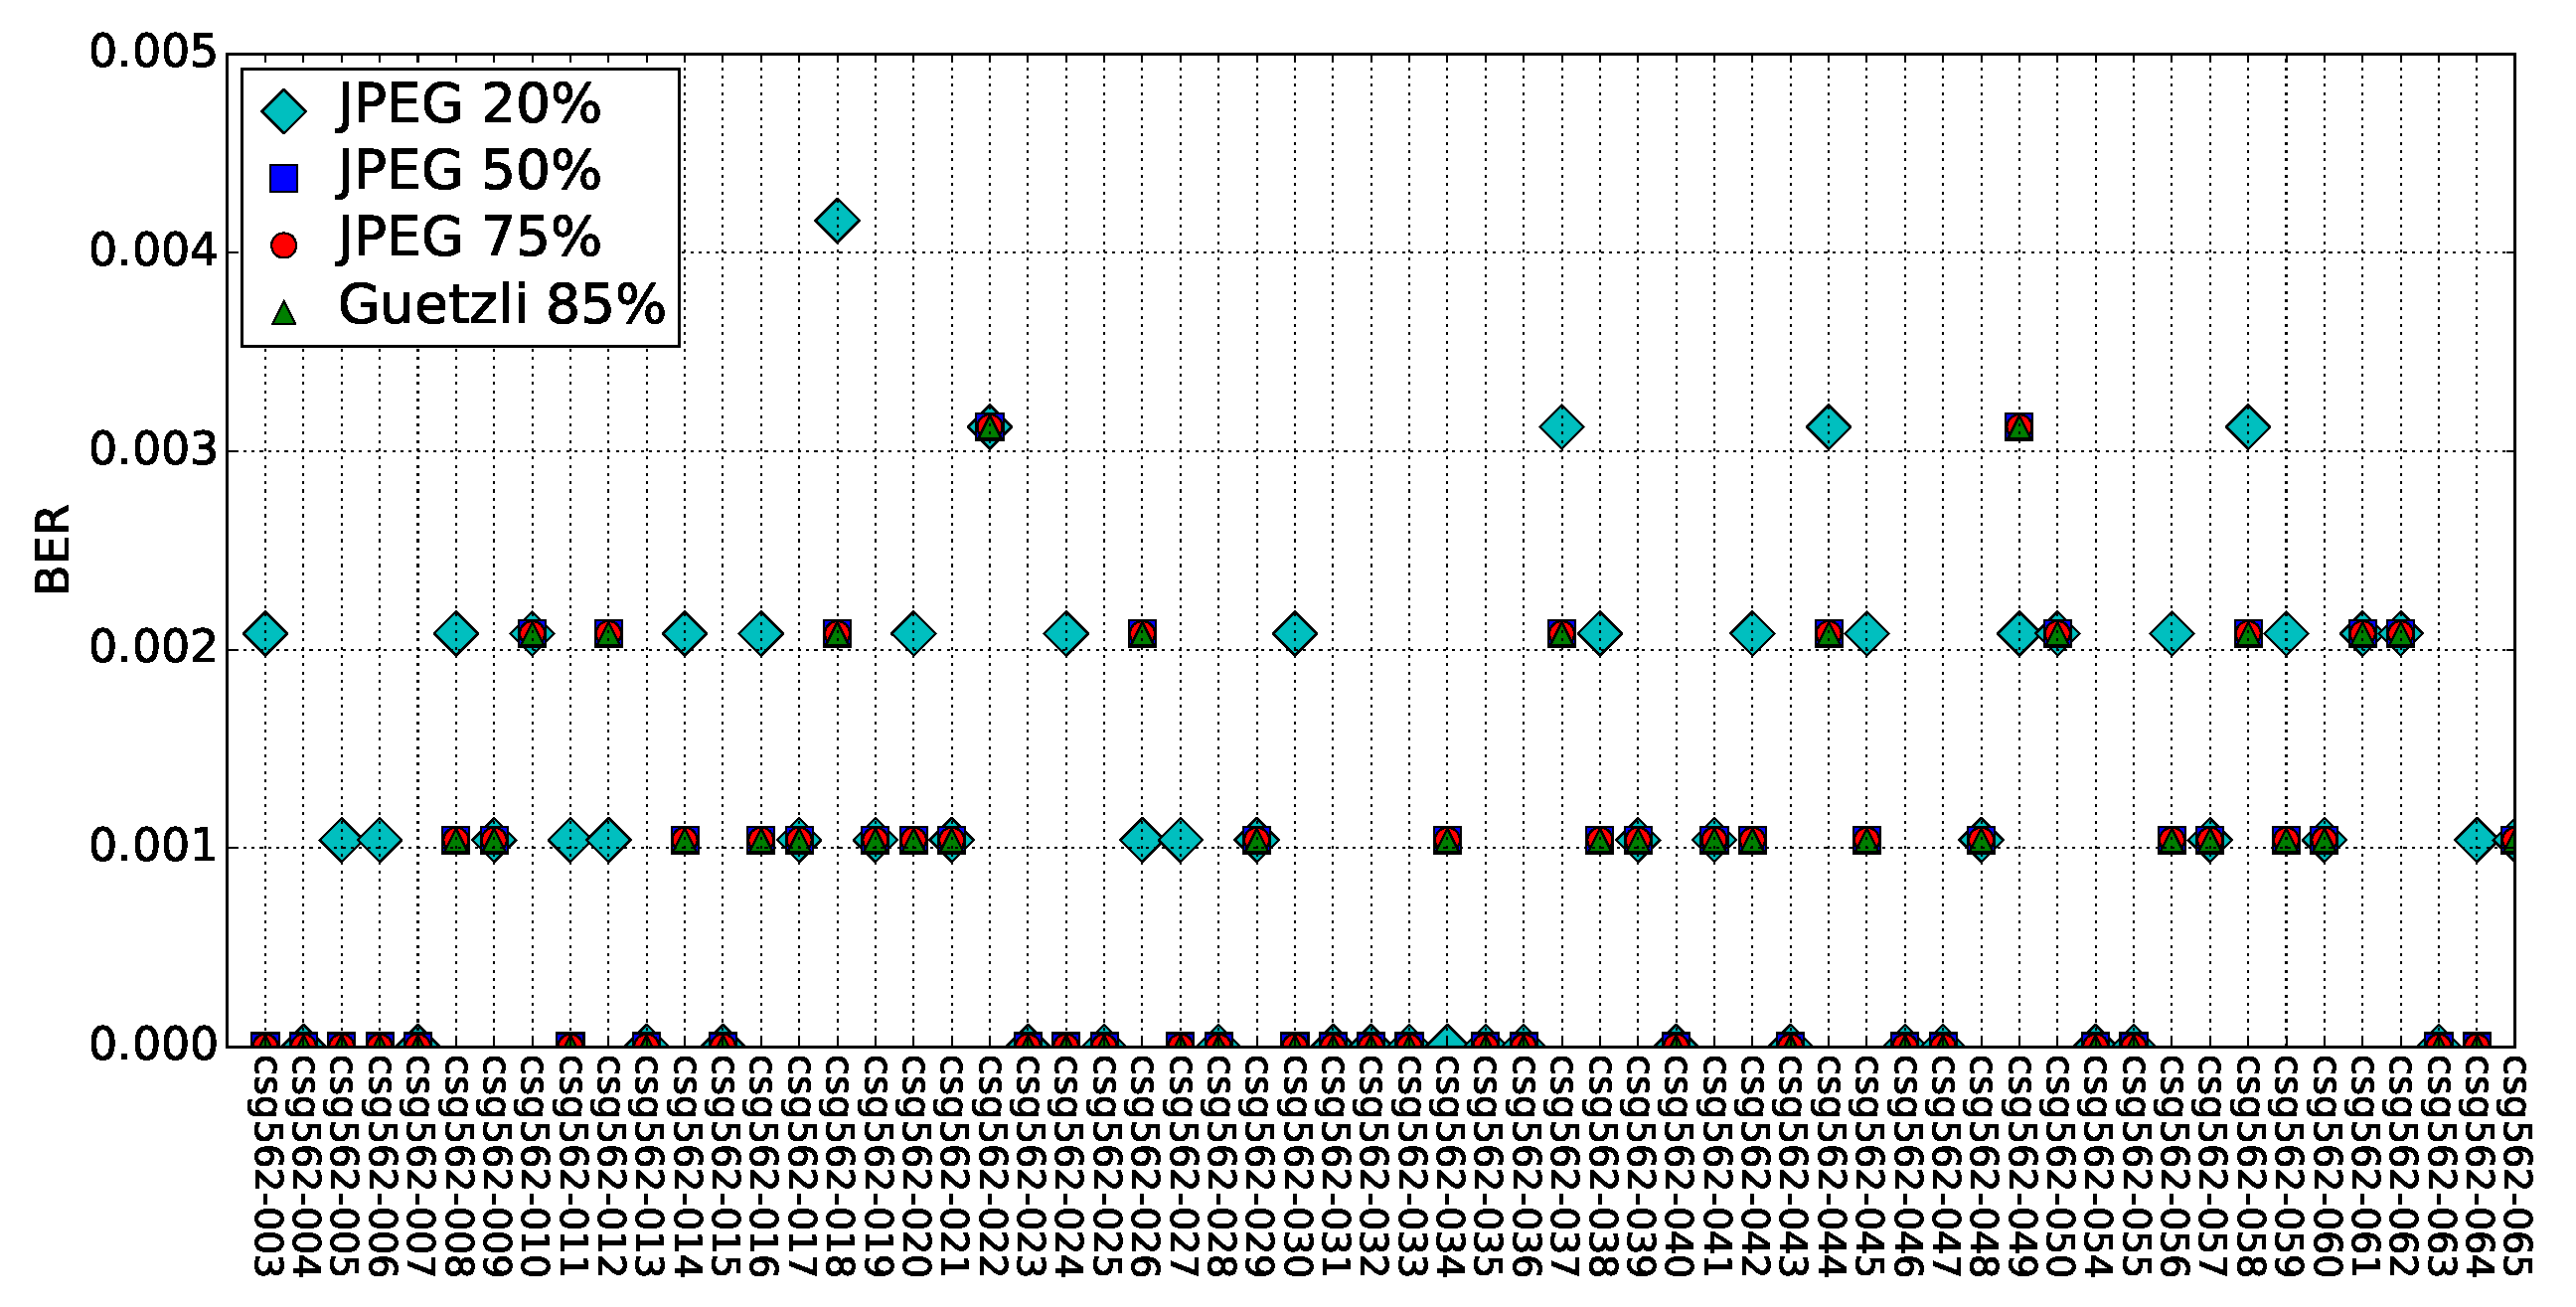
\includegraphics[width=0.86\textwidth]{ber.eps}
	\end{center}
	\caption{BER values under different JPEG compression attacks.}
	\label{ber}
\end{figure}
\section*{Conclusions}
In this paper, a digital watermarking technique based on Krawtchouk moments was implemented, and it was optimized by a genetic algorithm for manuscript document images. The results show a BER less than $0.005 \%$, so the extracted QR codes were decoded in $100\%$ of the $60$ analyzed images. In addition, the values of PSNR in all cases exceeded $44dB$. Thus, there is no visual difference between the original and watermarked images.

%
% the environments 'definition', 'lemma', 'proposition', 'corollary',
% 'remark', and 'example' are defined in the LLNCS documentclass as well.
%
%
% ---- Bibliography ----
%
% BibTeX users should specify bibliography style 'splncs04'.
% References will then be sorted and formatted in the correct style.
%
\bibliographystyle{splncs04}
\bibliography{mybibliography}
%

\end{document}
